\documentclass[../main.tex]{subfiles}

\begin{document}

\section{Cathodes}
\label{sec:cathodes}

\subsection{Introduction}
\label{sec:cathode_intro}
As mentioned in our Introduction (section~\ref{sec:intro}), lithium-ion batteries (LiBs) became promising applications in 1979 when Goodenough and Mizushima successfully demonstrated LiCoO$_2$ as a cathode.\cite{mizushima1980lixcoo2} Since then, LiBs have become instrumental in portable electronics, such as mobile phones, and electric vehicles, \cite{rozier2015li, whittingham2008materials, dunn2011electrical, liu2013materials,palacin2009recent} largely attributed to their high energy density. \cite{masquelier2013polyanionic,armand2008building,bruce2012li,park2010review,scrosati2011lithium,goodenough_li-ion_2013,etacheri2011challenges,takada2013progress,fergus2010recent,ellis2010positive,he2012layered,zaghib2013review} Due to the high abundance and low material cost, sodium-ion batteries have also received increased attention, especially for grid storage applications. \cite{ellis2012curr,kim2012electrode,palomares2012ion,fergus2012ion,yabuuchi2012p2} Regardless of the application, the discovery of new materials and the optimisation of current chemistries for improved performance is crucial for the next generation of rechargeable batteries. With that in mind, it is known that the energy density of the cathode material is the limiting factor in improving battery performance, thus current research is largely focused on exploring cathode chemistries. These include layered oxides (Li\textit{M}O$_2$, \textit{M}=Co,Mn,Ni), spinel oxides (Li\textit{M}$_2$O$_4$), olivine phosphates (LiFePO$_4$), disordered rock-salts, (Li$_2$MnO$_2$F), and other compounds, such as silicates. \cite{daniel2014cathode, islam2014lithium}

Layered transition metal (TM) oxides (Li\textit{M}O$_2$, \textit{M}=Co,Mn,Ni,etc.) are commonly considered to be the first generation of cathode materials in commercial LiBs. These materials possess a theoretical specific capacity of 270 mAh g$^{-1}$. However, their practical capacity is generally limited to below 200 mAh g$^{-1}$.\cite{myung2017nickel} \ce{LiCoO2} held high capacities but the material was problematic due to capacity fading, low abundance, and the high cost of cobalt and geopolitical issues, including ethical concerns, making large scale applications impractical. \cite{mo2018impact} There is also considerable instability in the LiCoO$_2$ structure, caused by the extraction of Li during cycling, which results in undesirable phase transitions from O3-type to O6-type Li$_x$CoO$_2$ and O1-type CoO$_2$. \cite{goonetilleke2018structural,chen2002staging} Other layered oxides also pose their own challenges, such as Li$_x$NiO$_2$ presenting capacity fade and poor safety, \cite{min2016comparative} and Li$_x$Mn$_2$O$_4$ presenting low capacity. \cite{tian2018performance} An emerging alternative to solve some of these challenges is using a combination of the TMs. In 2000, \citeauthor{paulsen2000o2} presented Li$_{2/3}$[Ni$_{1/3}$Mn$_{2/3}$]O$_2$, \cite{paulsen2000o2,paulsen20002} with Li[Ni$_x$Mn$_{1-2x}$Co$_z$]O$_2$ (NMC) presented by the authors in 2001. \cite{lu2001layered} Partially replacing Co in LiCoO$_2$ with Ni and Mn to obtain layered Li[Ni$_x$Mn$_y$Co$_z$]O$_2$, \cite{rozier2015li} where $x+y+z=1$, shows improved electrochemical performance, while also reducing material cost and improving stability.\cite{ohzuku2001layered} These layered oxides are commonly termed as NMC, with the subsequent numbering relating to the ratio between the cations.

A huge benefit of combining these TMs is the ability to tune the TM composition to optimise aspects including capacity, (dis)charging rate, electrochemical stability, and lifetime, with the potential of reaching capacities $>220$ mAh g$^{-1}$. \cite{duan2019insights} Some NMC compositions are already used commercially, with industry focus shifting from NMC111 to higher Ni containing compositions including NMC442, NMC532, and NMC622.\cite{zhang2018structural} These compositions, however, still contain 20 \% or more Co. A great deal of research is working towards reducing the Co content even further, with compositions such as NMC811 (Li[Ni$_{0.8}$Mn$_{0.1}$Co$_{0.1}$]O$_2$) showing promise as future commercial materials for applications, such as in long-range electric vehicles (EVs). \cite{azevedo2018mining} These Ni-rich NMC compositions are also considered to be the cathode of choice for future all-solid-state LiBs.\cite{myung2017nickel}

Recently, research into further improving the capacity of these materials by inserting lithium into the TM cation sites has attracted considerable attention. This has lead to a new generation of cathode materials termed ``Li-rich'' or lithium excess. The increased capacities of these materials arises from invoking redox chemistry on both the TM and oxide ions, as opposed to just TM ions in traditional oxide-based intercalation compounds. \cite{Sathiya2013,lee2014unlocking,Oishi2015,Seo2016,Gent2017,Assat2018,naylor2019depth,House2020,House2020a} These Li-rich cathodes, including Li$_{1+x}$Ni$_y$Co$_z$Mn$_{(1-x-y-z)}$O$_2$ layered oxide, can reach high capacities of $>300$ mAh g$^{-1}$. However, synthesis of these materials has proven to be difficult and work is ongoing to improve synthesis techniques.\cite{Hy2016} 

There has also been growing interest in disordered intercalation structures, especially disordered rock-salt structures. They were initially disregarded as cathodes, as their structure appeared to limit lithium diffusion. However, recent research has shown that lithium diffusion can be facile in some disordered materials, provided that there is enough of a lithium excess to allow the formation of an uninterrupted percolating network of channels involving no face-sharing TM ions.\cite{lee2014unlocking,Urban2014,Lee2015} There have been several examples reported, including Li$_{1.2}$Ni$_{0.33}$Ti$_{0.33}$Mo$_{0.13}$O$_2$,\cite{Lee2015} Li$_{1.2}$Ti$_{0.4}$Mn$_{0.4}$O$_2$,\cite{Yabuuchi2016a} Li$_4$Mn$_2$O$_5$,\cite{Freire2016,Yao2018,Bhandari2019454} Li$_3$NbO$_4$-based systems,\cite{Nakajima2017,Yabuuchi2015,Wang2015} and oxyfluorides, where some of the anion sites are occupied by F$^-$ rather than O$^2-$, such as Li$_2$MnO$_2$F,\cite{Sharpe2020,House2018,Lun2020} Li$_2$VO$_2$F,\cite{Chen2015,Chen2015a,Baur2019, Cambaz2019, Baur2020, Kallquist2019, Chang2020} and Li$_2$Mn$_{2/3}$Nb$_{1/3}$O$_2$F.\cite{Lee2018} These materials can be difficult to synthesise, however, as Mn-rich 3D TM compounds tend to form ordered phases, such as LiMnO$_2$ or Li$_2$MnO$_3$, high energy mechano-chemical ball-milling methods have been utilised to counter this.\cite{Freire2016,House2018,Freire2017} These materials are able to reach very high energy storage capacities of $300$ mAh g$^{-1}$,\cite{Jacquet2019} which is attributed to the ability to perform both cationic and anionic redox.\cite{Jacquet2019,clement2020,Chang2020} These materials typically show less first cycle hysteresis than other Li-rich compounds, thought to be because the structure already resembles that of the Li-rich materials after they undergo cation disorder on cycling.

\hlcyan{Knowledge of the broad structural and electrochemical properties of cathode materials can be obtained from various experimental methods. However, detailed insight into, for example, TM configurations, vibrational and thermal properties, and atomistic diffusion mechanisms, is challenging and, in some cases, not resolvable using experimental techniques. This is where atomistic modelling can provide greater insight.} In this section, we explore a range of cathode material properties, using several Li-ion materials, to highlight different properties and the considerations needed to gain the most desirable electrochemical performance. We describe which atomistic modelling methods are used to investigate the discussed properties and the importance of modelling in this context. Using a range of promising cathode materials (layered oxides, spinel oxides, polyanions, and disordered rock-salt oxides and oxyfluorides) to aid in the discussion, we first look at the different cathode crystal structures and the effects of micro-structuring. We then discuss some of the bulk material properties, including ion diffusion, redox and electronic properties, TM ordering, and vibration and thermal properties. Finally, we consider the surfaces and interfaces of these cathode materials, with an outlook to current and future challenges in the atomistic modelling of cathodes.

\subsection{Bulk Properties}
\subsubsection{Crystal Structure and Micro-Structure}
\textbf{Crystal structure}. Cathode materials consist of a range of different crystal structures, with some of the most promising LiCoO$_2$ based materials adopting the $\alpha$-NaFeO$_2$ structure, with alternating layers of [CoO$_2$]$^-$ and Li$^+$. In LiBs, the cathode is a limiting factor, as the amount of lithium that can be reversibly extracted and re-inserted (cycled) directly influences the battery capacity, with the Fermi energy linked to the cell voltage. \cite{islam2014lithium} Thermo-chemical stability and high energy density are also important considerations, with several promising candidates for future battery materials. These include mixed-metal layered oxides (NMC), spinel oxides (LiMn$_2$O$_4$), polyanion materials(LiFePO$_4$, \cite{whittingham2008materials,masquelier2013polyanionic,goodenough_li-ion_2013, zaghib2013review} Li$_2$FeSiO$_4$, \cite{nyten2005electrochemical,sirisopanaporn2011polymorphism,islam2011silicate} LiFeSO$_4$F \cite{padhi1997mapping}), and disordered rock-salt oxides and oxyfluorides (Li$_2$MnO$_2$F\cite{Jacquet2019, clement2020, Chang2020, Tygesen2020, Sharpe2020}). The crystal structures of these cathode materials are presented in Figures \ref{fig:cathode_structures} and \ref{fig:cathode_diffusion_pathways}, where these materials are described in more detail.

\begin{figure}
    \centering
    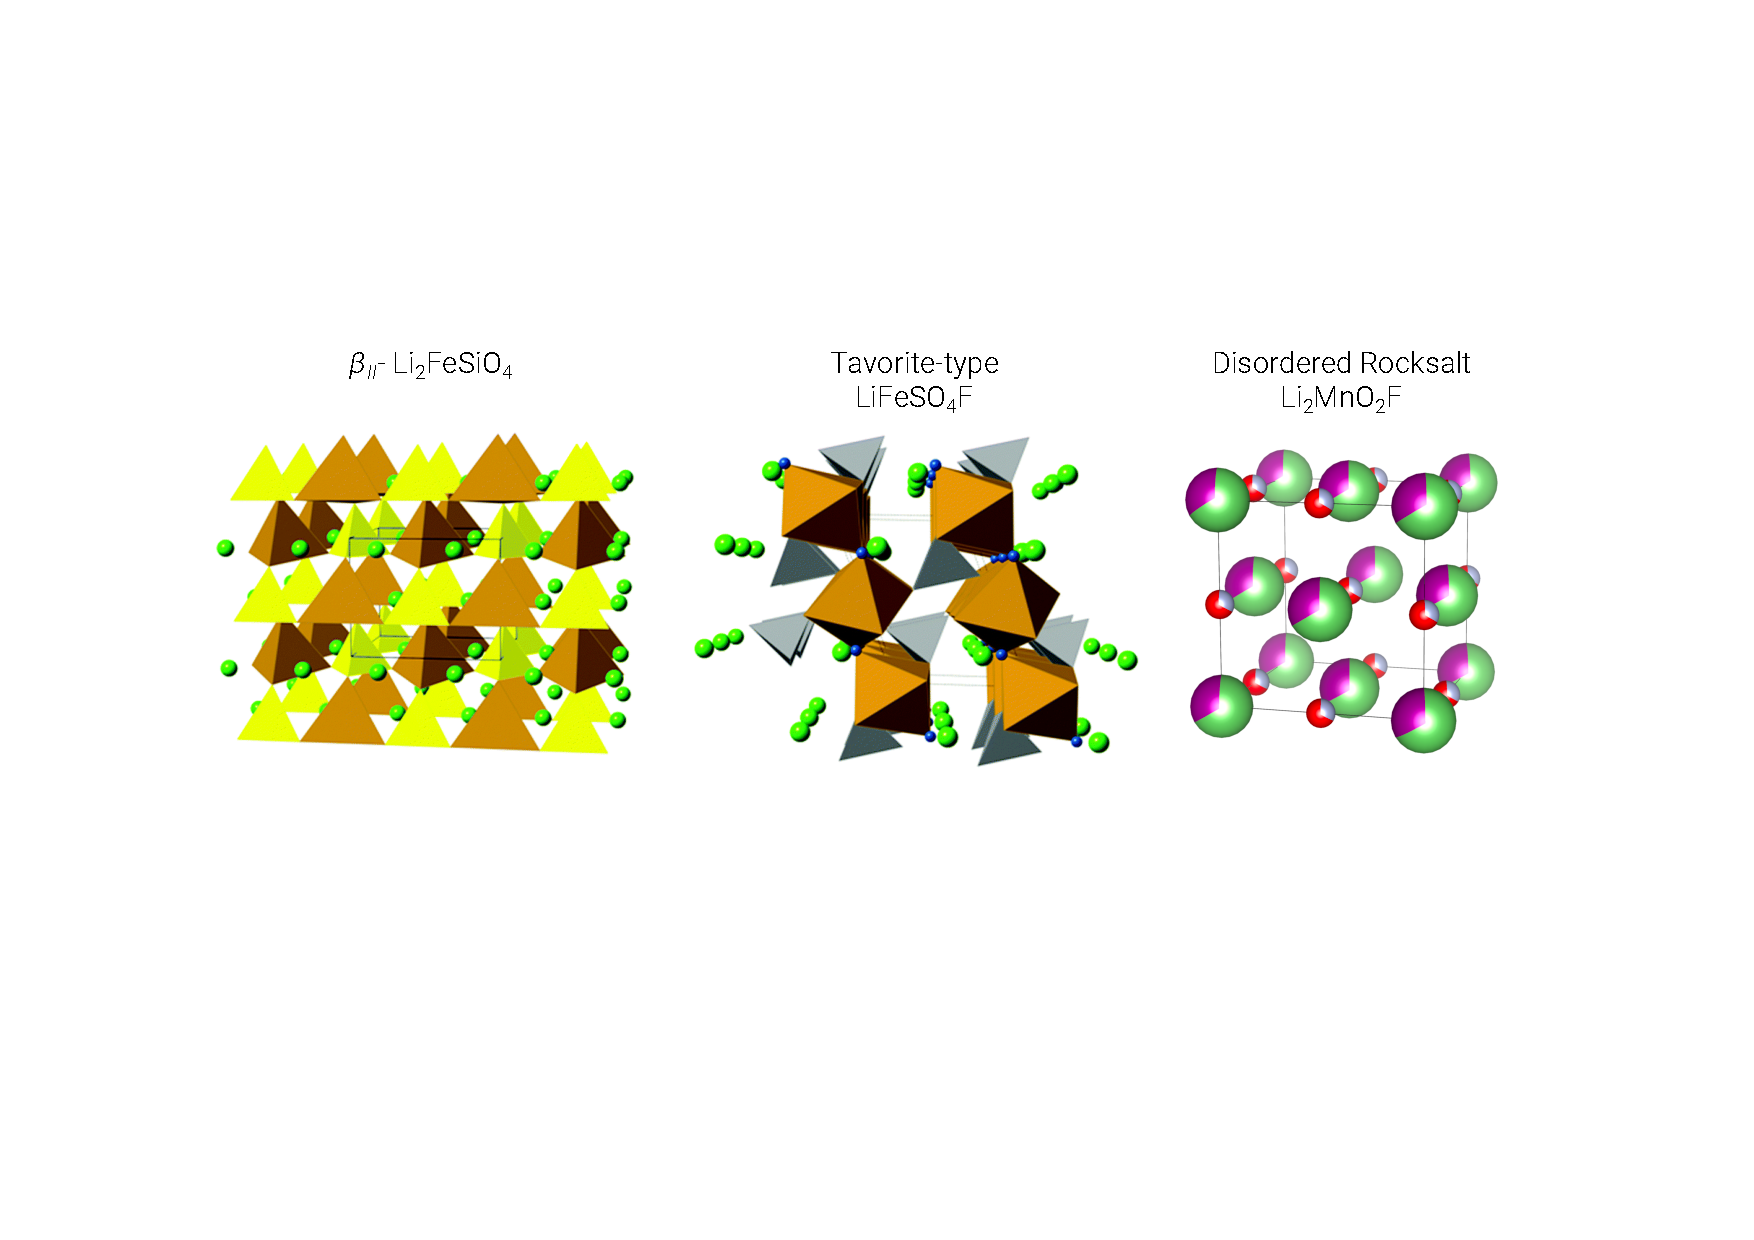
\includegraphics[scale=0.7]{figures/cathode_structures_others.pdf}
    \caption{Representative crystal structures of $\beta_{II}$-Li$_2$FeSiO$_4$, tavorite-type LiFeSO$_4$F, and disordered rock-salt Li$_2$MnO$_2$F cathode materials for lithium-ion batteries. Li$^+$ ions are shown in green spheres, O in red, Mn in mauve, and F in grey. Fe–O polyhedra are shown in brown, SiO$_4$ tetrahedra in yellow, and SO$_4$ tetrahedra in grey.}
    \label{fig:cathode_structures}
\end{figure}

Some TM oxides are stable in various structural forms, such as lithium manganese oxide (LMO), which has been synthesised with layered, \cite{armstrong1996synthesis} spinel, \cite{mosbah1983phases} and rock-salt structures. \cite{dittrich1969kristallstruktur} For intercalation-type cathodes used in LiBs, the structural framework is expected to remain relatively unchanged, with only small changes from lattice expansion/contraction. However, phase transitions can occur during the cycling process. For example, during cycling, a phase transition can occur from the LiMn$_2$O$_4$ spinel structure to the LiMnO$_2$ rock-salt structure, partially due to oxygen evolution. \cite{peng2017atomistic} Phase transitions between layered and spinel structures are also widely observed. \cite{chen2018understanding} For example, \citeauthor{reed2001layered} investigated the layered to spinel phase transitions in Li$_x$MnO$_2$ using Density Functional Theory (DFT) modelling (c.f. section~\ref{sec:dft}).\cite{reed2001layered} Their investigation determined that partially lithiated layered Li$_x$MnO$_2$ transitions to spinel in a two-stage process. Firstly, a large percent of Mn and Li ions quickly occupy tetrahedral sites, to form a meta-stable intermediate. Then, a more complex, coordinated rearrangement of Mn and Li occurs to form spinel. Interestingly, this behaviour is in contrast to Li$_x$CoO$_2$ and understanding the reasons for this could prove useful for creating Mn-based cathode materials.

\textbf{Micro-Structuring.} It is clear that control over bulk structure has an impact on the material's performance, as many properties are dependent on shape and size. \cite{bruce2008nanomaterials} The structural and micro-structural properties of a material are also vital to the cycling stability of a cathode. For example, reducing the particle size of LiFePO$_4$ to the nanometre scale is shown to increase the electrochemical performance, compared to equivalent, but larger, particles, by reducing transport path lengths.\cite{franger2006chemistry, ellis2007synthesis,malik2010particle} Selective structuring can also provide mechanical benefits, for example, where forces acting on the functional cathode during cycling, as the lattice expands and contracts with lithium intercalation, can cause plastic deformation and extinguish desirable activities. \citeauthor{sayle2018stress} modelled diffusion-induced stress in layered-spinel LMO composites, revealing structural resilience, enabled by flexing of a porous structure. \cite{sayle2018stress} In this study, \citeauthor{sayle2018stress} found the yield stress of the bulk material was 11.35 GPa, whilst the nanoporous material subjected to an equivalent strain experienced a stress of 4.32 GPa. In fact, it has been proposed that a $\beta$-MnO$_2$ host should be symmetrically porous and heavily twinned to maximise the cathode's electrochemical properties. \cite{sayle2009predicting} Further to this, intergrowing structures of two polymorphs of MnO$_2$, $\beta$-MnO$_2$ and Ramsdellite-MnO$_2$,\cite{Gupta2018} has been shown to enhance cell performance,\cite{GUPTA2020227619} due to reduction in stresses and facile diffusion in more open structure of Ramsdellite-MnO$_2$.

\subsubsection{Lithium-ion Diffusion}
\label{sec:cathode_ion_diffusion}
As discussed in section~\ref{sec:diffusion}, Li-ion diffusion coefficients can be calculated using multiple techniques, including \textit{ab initio} Molecular Dynamics (MD), classical (potentials-based) MD, and Monte Carlo (MC). Diffusion coefficients, although important experimentally and for parameterising continuum models, are not the only ion transport property of interest on the atomistic scale. Properties such as atomistic diffusion mechanisms, hopping frequencies, and activation energy barriers are all vital to understanding Li-ion transport and (dis)charge rate behaviour. This is of particular interest for investigating the effects of grain-boundaries and interfaces on the migration routes and mechanisms. For example, in LiCoO$_2$, \citeauthor{moriwake2013first} determined that the activation energy, $E_a$, for Li migration \textit{along} a twin boundary is 0.20 eV, smaller than that in the bulk, while the $E_a$ \textit{across} a twin boundary is 0.4 eV. \cite{moriwake2013first} This demonstrates the influence of grain-boundaries on the kinetic properties.

Computational techniques can provide information regarding a material's diffusion behaviour, which cannot be fully understood through experiments alone. For example, \citeauthor{dixit2015classical} compared Li and Na diffusion in Li$_{0.25}$FePO$_4$ and Na$_{0.25}$FePO$_4$, respectively, by calculating the potential and free energy diffusion barriers and determining the nuclear quantum effects (NQEs) of the Li ions.\cite{dixit2015classical} Their calculations found that Li diffusion was faster than Na diffusion, which is in agreement with experiments. However, the authors also determined that the NQEs for Li-ions were higher than those for Na-ions and that the quantum behaviour of the Li-ions was unusual. This information would not be possible to resolve using current experimental methods.

\begin{figure}
    \centering
    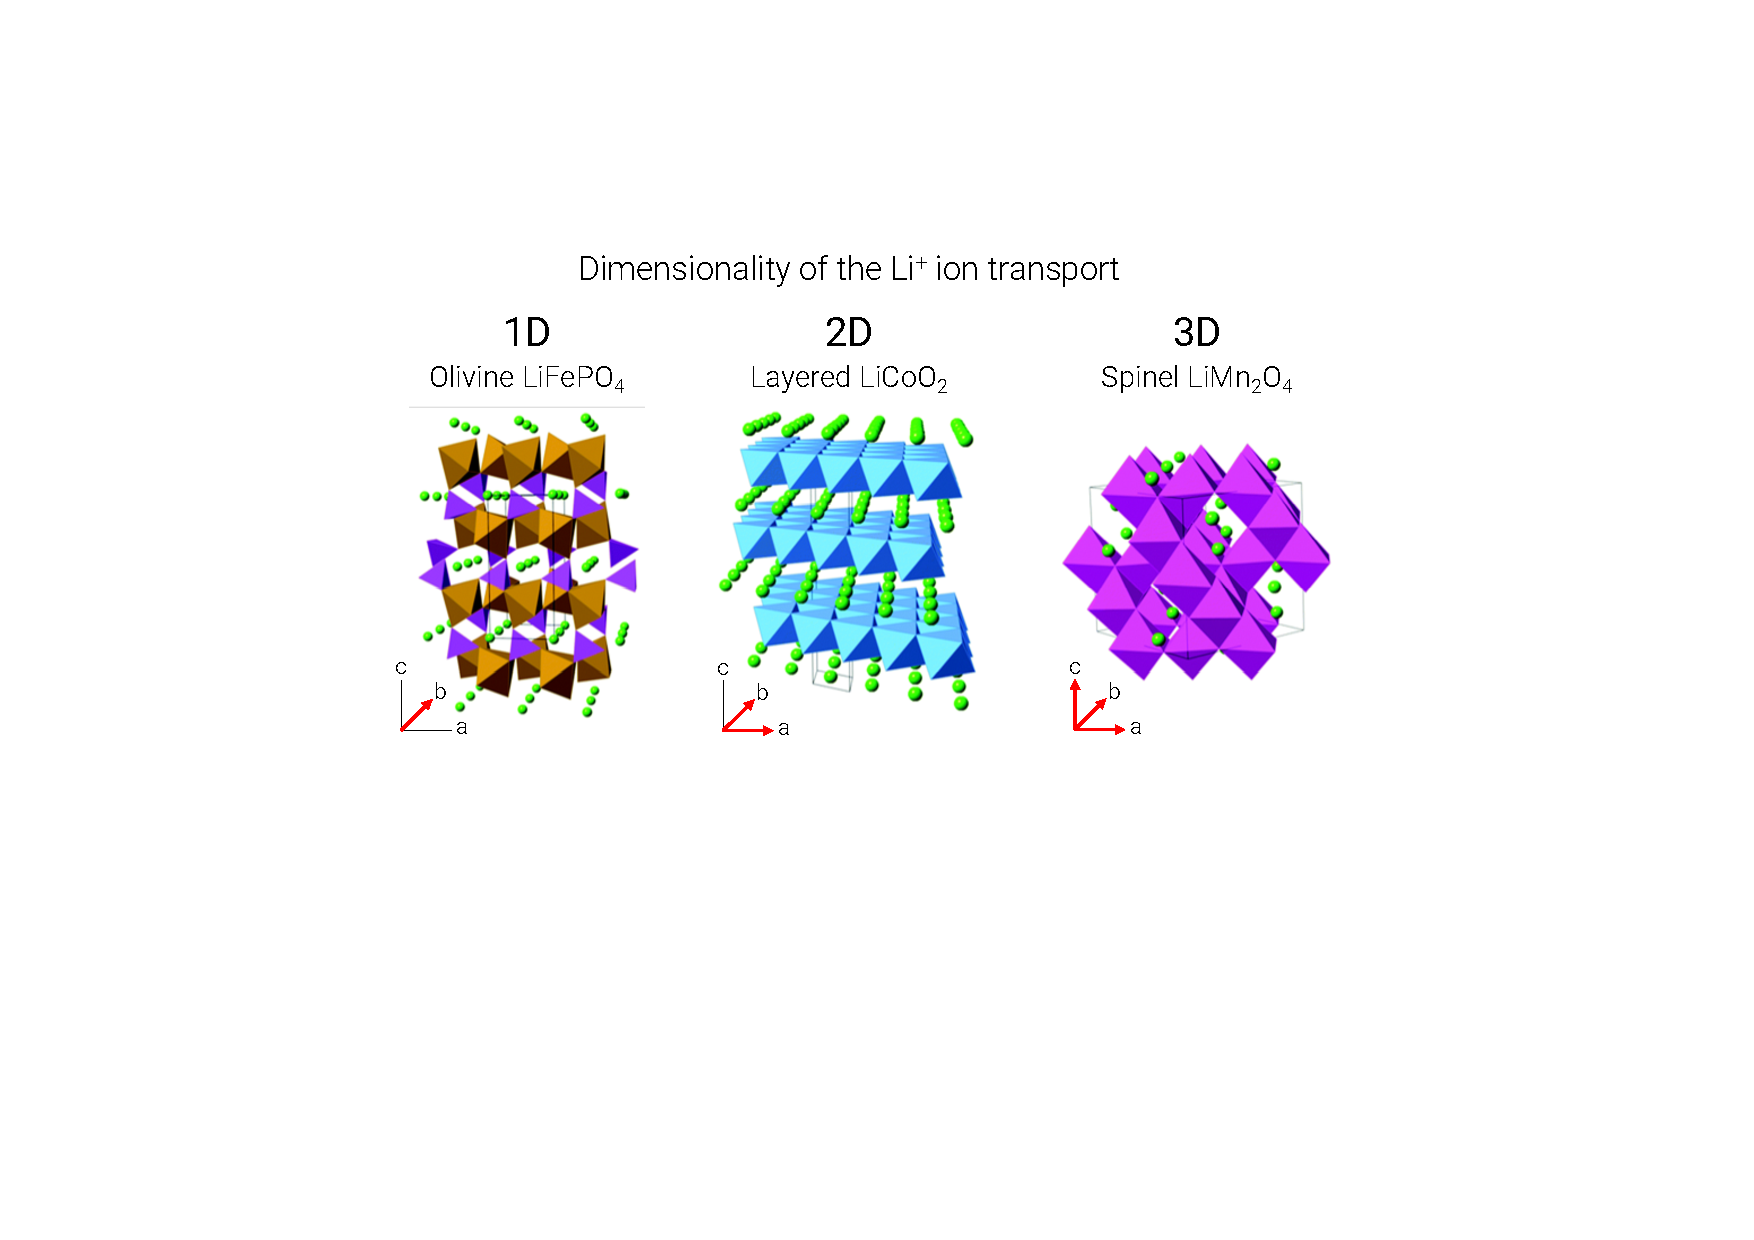
\includegraphics[scale=0.8]{figures/cathode_diffusion_pathways.pdf}
    \caption{Dimensionality of the Li$^+$ ion diffusion in LiFePO$_4$, LiCoO$_2$, and LiMn$_2$O$_4$. Figure edited and reproduced with permission from Ref.~\citenum{islam2014lithium} - Published by The Royal Society of Chemistry.}
    \label{fig:cathode_diffusion_pathways}
\end{figure}

The cathode crystal structure determines the available diffusion pathways in the material. DFT calculations\cite{Morgan2004,ouyang2004first} and classical MD using a core-shell model\cite{islam2005atomic} show Li$_x$FePO$_4$ is an olivine based structure which hosts Li over an interstitial network that has one-dimensional connectivity, i.e. 1-D diffusion, along the $b$ lattice vector of the orthorhombic cell.\cite{amin2006anisotropy} Li$_x$CoO$_2$ is a layered compound that accommodates Li ions within octahedral sites forming two-dimensional triangular lattices, resulting in 2-D diffusion, along the $b$ and $c$ lattice vector of the orthorhombic cell. \cite{van2000lithium} The spinel form of Li$_x$Mn$_2$O$_4$ has both tetrahedrally and octahedrally coordinated Li interstitial sites, forming a three-dimensional network and resulting in 3-D diffusion, along all lattice vectors. \cite{thackeray1997manganese,proell20123d} These different diffusion pathways can bee seen in Figure~\ref{fig:cathode_diffusion_pathways}. The 1-D diffusion pathways in Li$_x$FePO$_4$ are not actually exactly one dimensional. Although they travel solely along the $b$ lattice vector, the pathways themselves are curved, as shown in Figure~\ref{fig:curved_pathways}, as originally predicted by \citeauthor{islam2005atomic} using atomistic modelling,\cite{islam2005atomic} before later being observed experimentally.\cite{nishimura2008experimental}

\begin{figure}
    \centering
    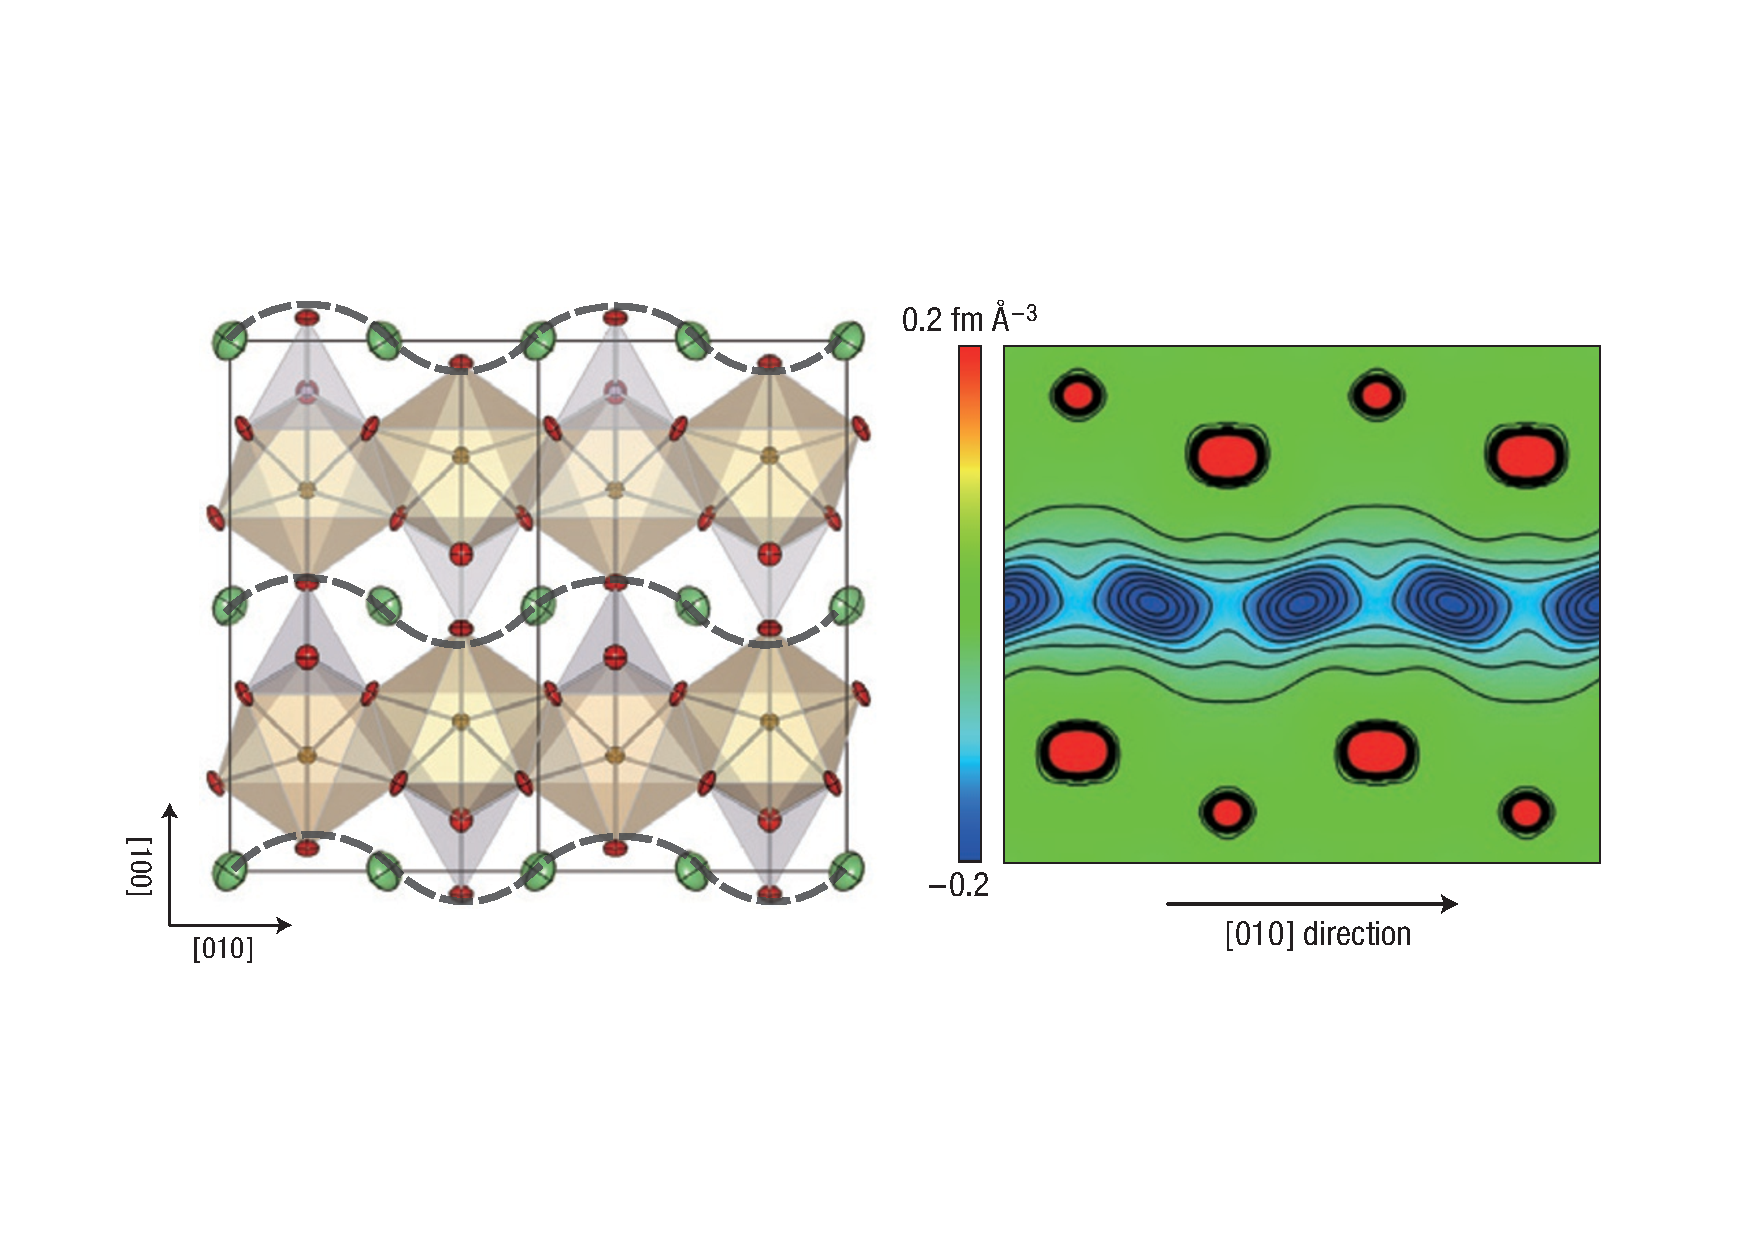
\includegraphics[scale=0.5]{figures/curved_1D_paths.pdf}
    \caption{Anisotropic harmonic lithium vibration in LiFePO$_4$. Expected curved one-dimensional continuous chains of lithium motion are drawn as dashed lines to show how the motions of Li atoms evolve from vibrations to diffusion. Two-dimensional contour map sliced on the (001) plane at z = 0.5; lithium delocalises along the curved one-dimensional chain along the [010] direction, whereas Fe, P, and O remain near their original positions.
    Adapted by permission from Springer Nature: Ref.\citenum{nishimura2008experimental}, Copyright 2008.}
    \label{fig:curved_pathways}
\end{figure}

Chemical diffusion coefficient of Li in an intercalation compound often has a strong dependence on Li concentration and crystal structure. The combination of DFT cluster expansion Hamiltonians with kinetic Monte Carlo (kMC) simulations, as described in sections \ref{sec:cluster_expansion} and \ref{sec:monte_carlo} revealed that the Li diffusion coefficients of TM oxides (and sulfides) are very sensitive to the Li concentration and also to the degree of cation ordering. \cite{van2008nondilute,VanderVen2001, bhattacharya2011first, bhattacharya2010phase, VanDerVen2013} For example, \citeauthor{VanderVen2020} shows the calculated Li diffusion coefficients for the layered (2D) and spinel (3D) forms of Li$_x$TiS$_2$ as a function of Li concentration. \cite{VanderVen2020,VanDerVen2013,van2008nondilute,bhattacharya2011first} This is presented in Figure~\ref{fig:LixTiS2_diffusion}, along with the structural images and vacancy mechanisms highlighted. Here it can be seen that not only do the Li diffusion coefficients differ by orders of magnitude, but the shape of the diffusion/Li concentration relation is very different. This shows how the crystal structure, and thus the active diffusion pathways, plays a crucial role in determining the concentration dependence of the diffusion coefficients in these materials.

\begin{figure}
    \centering
    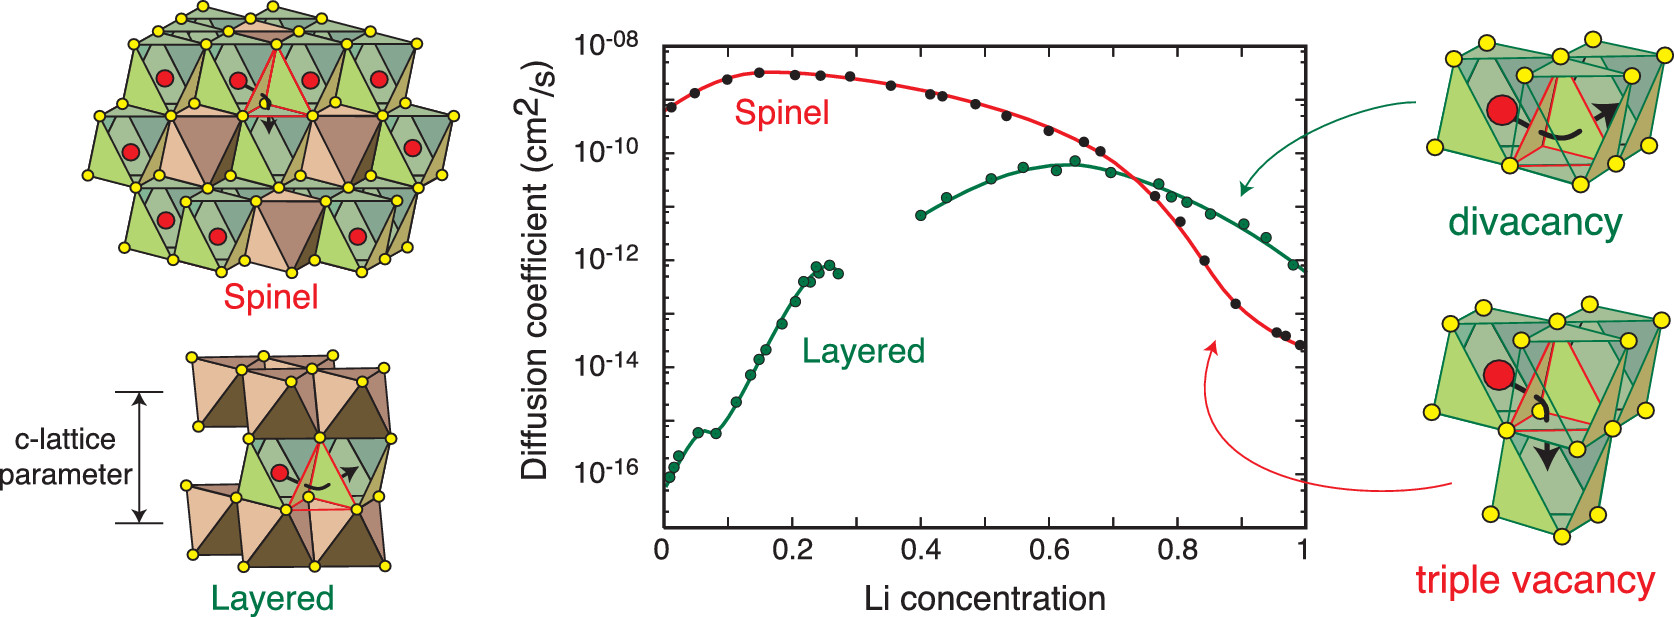
\includegraphics[scale=0.26]{figures/LixTiS2_diffusion.jpeg}
    \caption{Chemical diffusion coefficient of Li in an intercalation compound often has a strong dependence on Li concentration and crystal structure. Reprinted with permission from Ref.~\citenum{VanderVen2020}. Copyright 2020 American Chemical Society.}
    \label{fig:LixTiS2_diffusion}
\end{figure}

We have already eluded that diffusion is sensitive to the Li-ion concentration. However, the exact relation is through the activation barriers. Early DFT studies \cite{van2000lithium,van2001lithium} of Li$_x$CoO$_2$ systems showed that the lithium diffusion was predominately through a divacancy mechanism, when $0\leq x < 1$. However, at infinite vacancy dilutions diffusion is through a single vacancy mechanism. \cite{islam2014lithium} There are two hopping mechanisms at play here; oxygen dumbbell hops and tetrahedral site hops. Oxygen dumbbell hopping occurs when there is a single vacancy and a Li-ion has to travel between two occupied adjacent lithium sites to reach the vacant lithium site. Tetrahedral site hopping occurs when there are divacant or trivacant sites, i.e.  when one or both of the adjacent lithium sites are vacant. \cite{van2001lithium} Oxygen dumbbell hopping has a significantly lower migration barrier energy compared to tetrahedral site hopping, which highlights the sensitivity of the activation barrier to the lithium concentration. Experimental studies of mixed-TM layered oxides, such as Li(Ni$_{0.5}$Mn$_{0.5}$)O$_2$, have reported site exchange between Li and Ni ($\sim$ 8-12 \%).\cite{choi2005structural} DFT has been used to aid in understanding the effects of site--exchange on Li-ion mobility. \cite{kang2006electrodes,laubach2009structure} (De)intercalation of lithium in the material changes the distances between the layers. As Li is removed from the structure, there is a reduced ``barrier'' between the oxygen layers which start to repel one another. By calculating the activation energy as a function of the distance between the O layers on either side of the Li layers, a trend between increased O layer separation and lower activation energy is seen. \cite{kang2006electrodes,laubach2009structure}

In addition to the crystal structure and available diffusion pathways, doping the cathode material can also influence the material properties, including ion diffusion. NMC cathodes are effectively LiCoO$_2$ doped with Ni and Mn. As previously mentioned in section \ref{sec:cathode_intro}, introducing Ni and Mn into the system to form a mixed-TM layered oxide increases the diffusion/conductivity and electrochemical performance. There are very few detailed computational studies of mixed-TM oxides due to their complexities. An illustration of this is the complexities which arise from TMs, such as Fe, Ni, Co, and Mn, which exhibit localised oxidation states. This can be further complicated, or influenced by, TM ordering. For instance, \citeauthor{lee2013solid} investigated the effects of TM disorder on the electrochemical properties of Li$_x$Ni$_{0.5}$Mn$_{1.5}$O$_4$ using cluster expansion and MC methods (c.f. sections~\ref{sec:cluster_expansion} and \ref{sec:monte_carlo}). The authors determined a correlation between Li vacancy ordering and TM ordering.\cite{lee2013solid} \citeauthor{hao2016quaternary} found similar evidence for Li$_x$(Mn$_y$Ni$_{1-y}$)$_2$O$_4$.\cite{hao2016quaternary} These also have an effect on the diffusion properties of the material. TM ordering in NMC cathodes is discussed in more detail in section \ref{sec:TM_ordering_NMC}. Using experimental techniques, \citeauthor{capsoni2002inhibition} found that doping the cationic sublattice of spinel LiMn$_2$O$_4$ with as low as 1 \% Ga${^3+}$ significantly modifies the temperature of the conductivity drop associated with Jahn-Teller (JT) distortion, preventing the transition observed near room temperature. \cite{capsoni2002inhibition} This allows for a wider temperature window for the higher conductivity phase. DFT using generalised gradient approximation (GGA) or its variant GGA+U (c.f. section~\ref{sec:dft}), was also employed to analyse the effect of doping LiMn$_2$O$_4$ on the JT distortion. In this study, \citeauthor{singh2009suppression} found that doping with Cr and Mg also suppressed the JT distortion and thus the associated temperature of the conductivity drop.\cite{singh2009suppression} 

\subsubsection{Redox and Electronic Properties}
The cathode operates by the deintercalation of Li$^+$ on charging, and the reinsertion of Li$^+$ on discharging. The charge is balanced by the oxidation and reduction of the TM ion, e.g. LiCo$^{3+}$O$_2$ $\rightleftharpoons$ Li$_{1-x}$Co$^{4+}$O$_2$ + $x$Li$^+$ + $x$e$^-$. 
The role of TM redox in LiBs has been well known since the first publications by Goodenough on LiCoO$_2$ as an intercalation electrode in 1980.\cite{mizushima1980lixcoo2} Although various classes of compounds have been investigated over the years, the overall mechanism of TM redox is broadly similar. The three major classes of oxide cathodes, (layered,\cite{mizushima1980lixcoo2} polyanion,\cite{padhi1997olivine} and spinel\cite{Thackeray1983}) all function via a TM redox couple. The specific capacity of most LiB cathode materials is limited by the number of electrons per TM cation that can participate in the redox reaction. However, the recent discovery of oxygen redox reactivity, O$^{2-}$ $\to$ (O$_2$)$^{n-}$,  in Li-excess cathode materials\cite{Koga2013, Sathiya2013, Oishi2015, Sathiya2015, McCalla2015, Cao2015, Shimoda2016, Chen2016, Luo2016a, Hy2016, Muhammad2016, Seo2016, Gent2017, Zhan2017,  Zheng2017,Assat2018, BenYahia2019, naylor2019depth, Hua2019, House2020, Li2019, Eum2020, Gent2020, Sharpe2020} has prompted further investigation.

\hlcyan{DFT has been pivotal in shedding light on this phenomenon, in conjunction with a range of experimental techniques. DFT can be used to analyse the atomic charge and electronic structure of each ground state, enabling the charge compensation during delithiation to be correctly attributed during simulated charging.} \citeauthor{Yao2018} were able to propose a sequence of redox events for delithiation of Li$_4$Mn$_2$O$_5$;\cite{Yao2018} first, cationic redox, Mn$^{3+}$/Mn$^{4+}$, dominates for Li$_x$Mn$_2$O$_5$, when 4 $\geq$ x $>$ 2. Then anionic redox, O$^{2-}$/O$^{1-}$, dominates for Li$_x$Mn$_2$O$_5$, when 2 $\geq$ x $>$ 1. Finally, mixed cationic (Mn$^{4+}$/Mn$^{5+}$) and anionic (O$^{2-}$/O$^{1-}$) redox for Li$_x$Mn$_2$O$_5$, when 1 $\geq$ x $\geq$ 0. Meanwhile, fluorinated materials such as Li$_2$Mn$_{2/3}$Nb$_{1/3}$O$_2$F\cite{Lee2018} and Li$_2$MnO$_2$F\cite{Sharpe2020} were found to exhibit some overlap between the redox processes, suggesting that the substitution of O by F favours lower Mn oxidation states, therefore leading to more redox overlap with oxygen. \hlcyan{DFT has also been used to establish the band structure for cathode materials, determining which TM orbitals hybridise more with the O(2p) orbitals}\cite{Cao2015, Sathiya2013a} \hlcyan{and to identify hole states.}\cite{Zhan2017, Xiao2012}

In a combined experimental and computational study, \citeauthor{Gent2017} observed a strong correlation between anion redox, cation migration, and open circuit voltage (OCV) hysteresis in Li-rich layered oxides.\cite{Gent2017} \citeauthor{Hong2019} offered an explanation for the strong coupling between anion redox and structural disordering in Li rich layered oxides; they found local stabilisation of short $\sim$1.8 \AA \ metal-oxygen $\pi$ bonds and $\sim$1.4 \AA \ O-O dimers during oxygen redox.\cite{Hong2019}

\citeauthor{Seo2016} showed that anion redox chemistry is heavily dependent on the anion nearest-neighbour coordination environment.\cite{Seo2016} In particular, they described how more Li-O-Li configurations lead to more potentially labile oxygen electrons, resulting in enhanced O redox chemistry, as shown in Figure~\ref{fig:o_redox}. A similar result was found with Li$_2$MnO$_2$F; those oxygens coordinated to at least five Li (e.g. OLi$_5$Mn) in the fully lithiated state were the first to oxidise, whereas those coordinated to three or fewer (e.g. OLi$_3$Mn$_3$) did not undergo oxidation at all. This showcased a more continuous variation in the O-redox potential, dependent on the number of Li coordinated to a given O$^{2-}$ ion.\cite{Sharpe2020} \hlcyan{Recent computational screening work on layered oxide cathodes using hybrid DFT has reported trends in O-redox activity associated with the electrostatic (Madelung) energy at oxygen sites.}\cite{Davies2020}

\begin{figure}
    \centering
    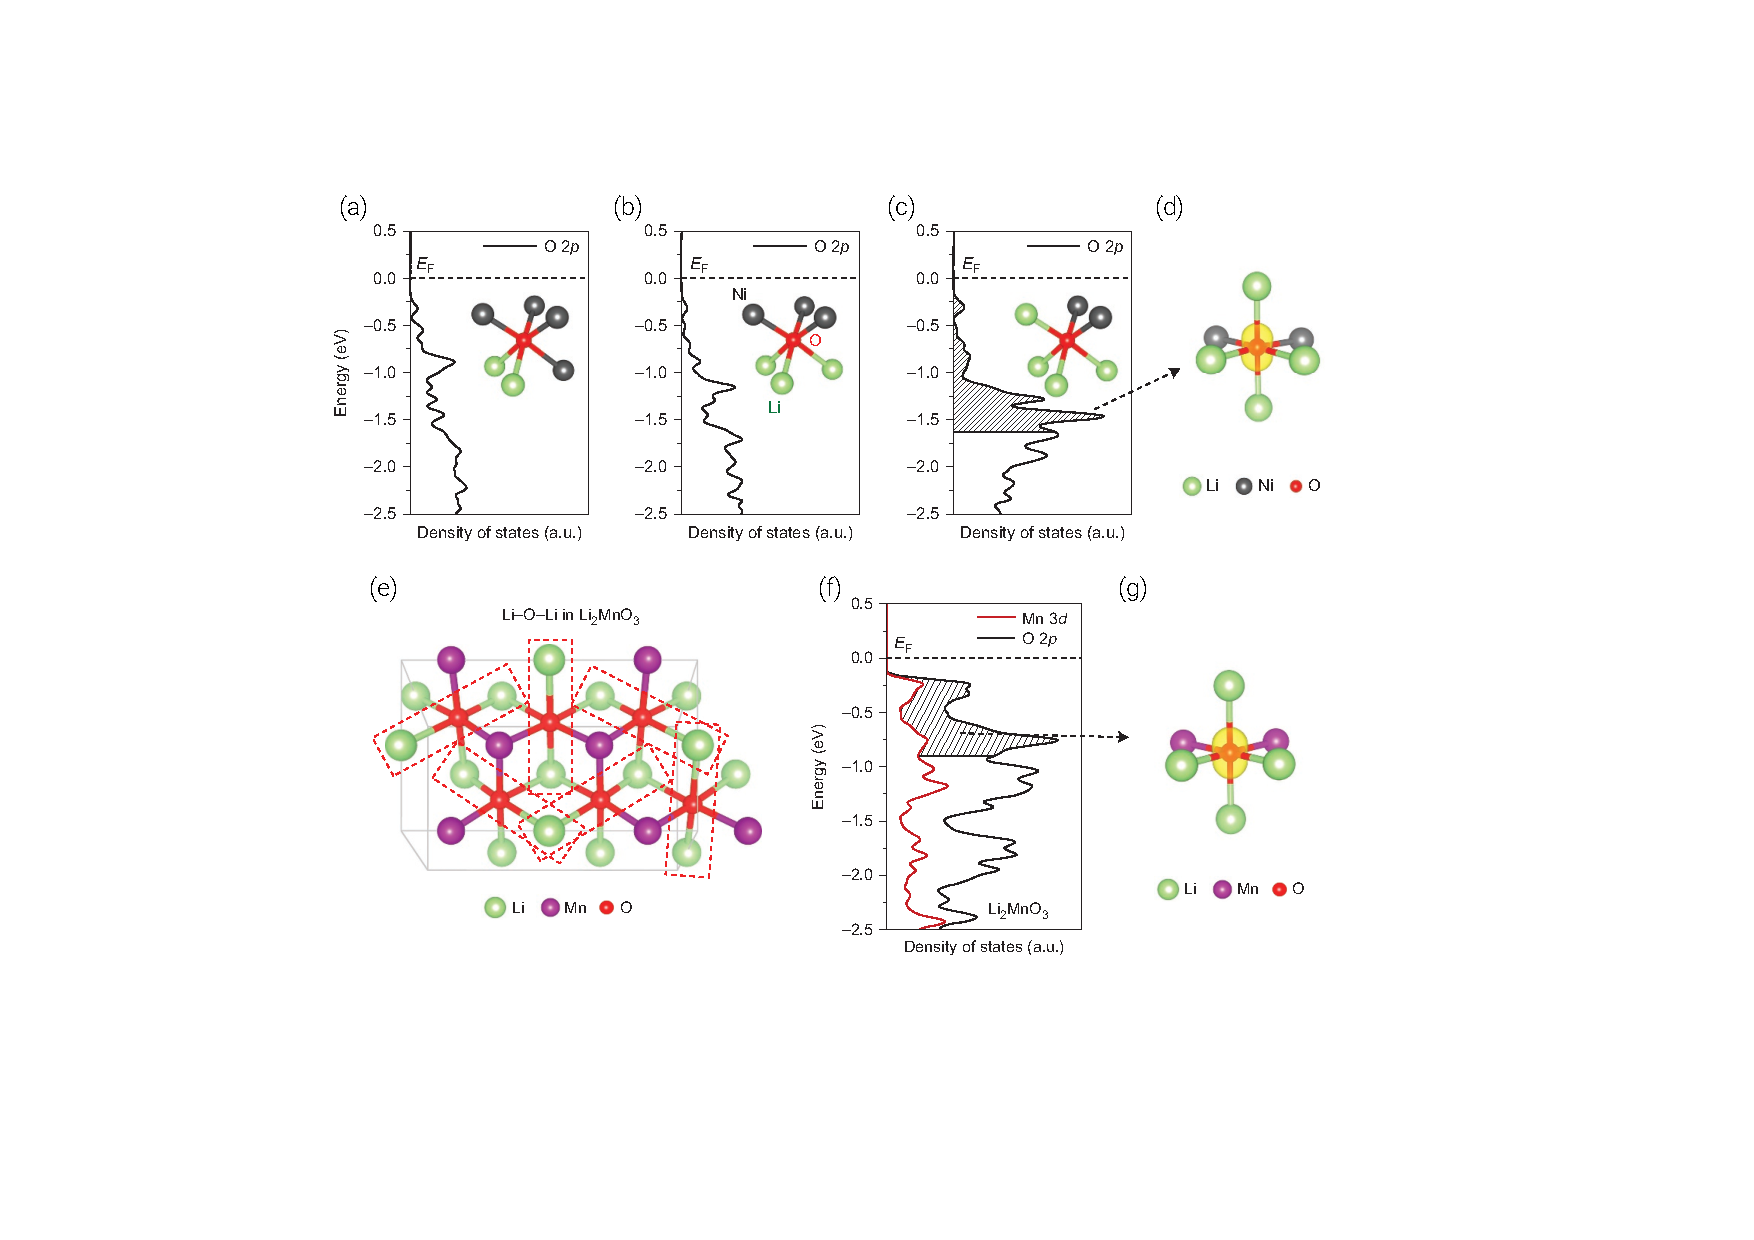
\includegraphics[scale=0.7]{figures/o_redox.pdf}
    \caption{ Effect of local atomic environments on the electronic states of O ions in (a-d) cation-mixed layered LiNiO$_2$ and (e-g) Li$_2$MnO$_3$. Cation mixing introduces various local environments around oxygen. Projected density of states (pDOS) of the O $2p$ orbitals of O atoms in cation-mixed layered LiNiO$_2$ coordinated by (a) two Li and four Ni, (b) three Li and three Ni, and (c) four Li and two Ni. (d) gives the isosurface of the charge density (yellow) around the oxygen coordinated by four Li and two Ni, in the energy range of 0 to -1.64 eV. (e) gives an illustration of Li-O-Li configurations in Li$_2$MnO$_3$, with (f) giving the related pDOS of the O $2p$ orbitals and Mn $3d$ orbitals, and (g) giving the isosurface of the charge density (yellow) around the oxygen, in the energy range of 0 to -0.9 eV. Adapted by permission from Springer Nature: Ref.\citenum{Seo2016}, Copyright 2016.}
    \label{fig:o_redox}
\end{figure}

\citeauthor{Chen2016} investigated delithiation and kinetic processes in Li$_2$MnO$_3$ using hybrid DFT and found that Li extraction is charge-compensated by oxidation of the oxide anion, so that the overall delithiation reaction involves lattice oxygen loss.\cite{Chen2016} Localised holes on oxygen (O$^-$) are formed at the first step but, due to their instability, lead to oxygen dimers (O-O is approximately 1.3 \AA) and eventually to the formation of molecular O$_2$. This then facilitates Mn migration to the octahedral site in the vacant Li layer, leading to a spinel-like structure. DFT has also been used to show the formation of O$_2$ at high states of charge in Li$_2$MnO$_2$F\cite{Sharpe2020} and Li$_{1.2}$Ni$_{0.13}$Co$_{0.13}$Mn$_{0.54}$O$_2$, \cite{House2020a} agreeing with experimental resonant inelastic X-ray scattering (RIXS) data, and to report superoxide formation in Li$_2$VO$_2$F, in agreement with electron paramagnetic resonance (EPR) spectroscopy studies.\cite{Chang2020}

\subsubsection{TM Ordering in NMC Layered Oxides}
\label{sec:TM_ordering_NMC}
Cation/anion ordering also plays a vital role in the properties/activity of a material, such as the physical and electrochemical properties. A topical illustration of this is the NMC cathode materials, where recent experimental studies show that spin interaction of the TM ions is a major challenge.\cite{duan2019insights, xiao2018insight} The varying compositions, charge distributions, and electronegativities of the TMs lead to a mixture of valence states, where Ni can exist as Ni$^{2+}$, Ni$^{3+}$, and Ni$^{4+}$, Co can exist as Co$^{3+}$ and Co$^{4+}$, and Mn exists as Mn$^{4+}$.\cite{xiao2018insight} The interactions between these mixed valence states poses a challenge to the identification of ground states. As NMC materials, such as NMC811, emerge as front runners for commercialisation, research into their specific chemistry has become of great interest. \hlcyan{Recently, several computational studies have been performed to analyse the influence of TM valence states on the stability and structure-property relationships of NMC materials, which are challenging to resolve experimentally.}\cite{sun2017electronic,dixit2017origin, hoang2016defect,dixit2017unraveling} \hlcyan{For example,} \citeauthor{sun2017electronic} \hlcyan{analysed 81 NMC compositions using DFT, observing that random arrangements of TMs present similar thermodynamic states.}\cite{sun2017electronic} \hlcyan{Clusters of random geometries and population were seen, which confirmed that no specific ordering exists at the superlattice scale. This is consistent with previous experiment analysis using X-ray and neutron diffraction characterization on a specific composition of NMC, Li$_{2/3}$[Co$_x$Ni$_{1/3-x}$Mn$_{2/3}$]O$_2$, demonstrating that Co suppresses the superlattice ordering when $x > 1/6$.}\cite{lu2000superlattice} \hlcyan{The authors also demonstrated, through intensive computational screening, that no long-range ordering exists in the TM layer of NMC. These DFT studies provide fundamental understanding of the physicochemical properties at the intrinsic level of electronic structures and will offer important insight in the selection of NMC materials for enhanced electrochemical performance. It would not be tractable to analyse so many compositions of NMC through experiments.}

\subsubsection{Vibrational and Thermal Properties}
An important contribution to the thermodynamic properties at finite temperature is the vibrational partition function, which can be evaluated by calculating the material’s normal modes of lattice vibrations. A number of researchers have theoretically addressed the vibrational contribution to the material thermodynamic properties in LiBs, especially in NMC cathodes.\cite{du2016insight,yang2019highly,yang2020chemical} There are several works studying cathode materials beyond NMC. \citeauthor{shang2012lattice} employed DFT phonon calculations with a mixed-space approach to probe the lattice dynamics and finite-temperature thermodynamic properties of olivine structure \ce{LiMPO4} (M = Mo, Fe, Co, Ni).\cite{shang2012lattice} The authors reported that \ce{LiMPO4} structures from Mn, Fe, Co, to Ni show increasing zero-point vibrational energy, but a diminishing vibrational contribution to the Gibbs energy, due to the decreasing phonon densities of state at the low frequency region of \ce{LiMPO4}. Recently, lattice dynamics studies have been expanded to solid electrolytes, aiding in the discovery of lithium fast-ion conductors.\cite{sagotra2019influence} 

Two major approaches have been developed to compute lattice thermal conductivity; by solving the Boltzmann transport equation (BTE) using anharmonic lattice dynamics and through MD simulations. \citeauthor{puligheddu2019computational} compared lattice thermal conductivity values from these two methods and found a satisfactory agreement.\cite{puligheddu2019computational} The comparison used empirical potentials and took into account the effects of both fourth order phonon scattering and temperature-dependent phonon frequencies, reporting the different effects of quantum and classical statistics.

Using BTE within the relaxation-time approximation, \citeauthor{mattila2020lattice} reported the highly anisotropic lattice thermal conductivities in isotopic \ce{LiCoO2}, close to the values in \citeauthor{yang2019highly}'s work\cite{yang2019highly,yang2020chemical}, and illustrated the effect of the alkali metal atom by replacing Li by Na.\cite{mattila2020lattice} The authors explained this through the significantly shorter phonon lifetimes in \ce{LiCoO2}. They found that in-plane lattice thermal conductivities in \ce{NaCoO2} are $\sim$0.7 times larger than that in \ce{LiCoO2} at room temperature, since the former has significantly longer phonon life times. While \citeauthor{feng2020quantum} report much lower thermal conductivity values by including four-phonon scattering, using a different functional, the local density approximation (LDA), for exchange and correlation.\cite{feng2020quantum} They also investigated the thermal transport reduction during delithiation (charging) due to reduced phonon velocities and increasing anharmonicity. Furthermore, grain-boundary effects reduced thermal transport and suppressed thermal conductivites in polycrystals are well reproduced when grain sizes were reduced down to several nm in either BTE or MD simulations. \cite{he2019thermal}

The thermal conductivity investigation can be also performed on anodes and many other materials.\cite{qian2016anisotropic, wei2018tunable} Recently, a high-throughput study was reported for 37 binary rock-salt and zinc blende material systems, in which the authors highlight the importance of high-order phonon-phonon interactions based on harmonic calculations.\cite{xia2020high} \hlcyan{Modelling heat transport using DFT calculations is complex but essential due to the difficulties inherent in preparing high-quality samples for experimental measurements.}

\subsection{Surfaces}
\hlcyan{Surface structures and morphologies of cathode particles can be difficult to determine using experimental microscopy and spectroscopy methods alone and thus computational investigations can provide vital insights.}\cite{zhang2013nanomaterials} \hlcyan{Due to their synthesis conditions, experimental cathode materials comprise different surface facets, defects, and particle sizes. It is therefore necessary to use model systems to determine which of these effects is more important by studying them in isolation, separating the effects, which is not possible using experimental materials.} Both \textit{ab initio} and potentials-based MD have been extensively used to investigate the surfaces and morphologies of layered oxides, spinel oxides, and olivine phosphates, which will be briefly discussed here. These techniques have also been used to investigate cathode materials in sodium-ion batteries, which is covered in more detail in Ref.~\citenum{islam2014lithium}.

With oxides at the forefront of the battery revolution, it is unsurprising that there have been many DFT and potentials-based MD studies into layered LiCoO$_2$, LiMn$_2$O$_4$ spinel, MnO$_2$-type and related materials, looking at properties including the surfaces, nanostructures, and morphologies.\cite{kramer2009tailoring,xu2011identifying, daheron2009surface,kim2012first,benedek2011simulation,karim2013surface,leung2012first, tompsett2013nanostructuring} Surface energies for low-index layered LiCoO$_2$ surfaces, as a function of external Li and O chemical potentials, revealed the (0001) and (10\={1}4) surfaces were present for all reasonable values of Li and O chemical potentials, whereas the (01\={1}2) surface was only stable under oxidising conditions.\cite{kramer2009tailoring} Studies into the low-index surface facets of LiMn$_2$O$_4$ determine the (111) surface to be the most stable. This is due to the site exchange of under-coordinated Mn on the surface, which exhibit a cubo-octahedral type, predominately comprising \{111\} surfaces. \cite{karim2013surface} Other studies show that the Mn-terminated (111) surfaces undergo surface reconstruction, indicating instead that the Li-terminated (001) surface has the lowest energy.\cite{benedek2011simulation}

It has also been shown that electronic spin state transitions occur on the surfaces of stoichiometric LiCoO$_2$. Here \citeauthor{qian2012electronic} found that the trivalent Co ions at the surface adopt an intermediate spin state if they are square–pyramidally coordinated and a high spin state if they are pseudo-tetrahedrally coordinated. This highlighted the effect of low-coordinated geometries at the particle surface on the Co$^{3+}$–Co$^{4+}$ redox potential.\cite{qian2012electronic} \citeauthor{hong2019electronic} investigated the surface properties of LiCoO$_2$ nanoplatelets and their chemical modifications with Al$^{3+}$, using combined experimental and theoretical approaches.\cite{hong2019electronic} Their models also showed the electronic structures of several LiCoO$_2$ surface facets are different from those of the bulk, attributing this to the altered spin states of surface Co$^{3+}$ atoms. The authors found splitting of the Co 3d–O 2p states, which were linked with high-spin-state Co$^{3+}$ at the surface. Partial substitution of Co$^{3+}$ by Al$^{3+}$ was found to increase the ratio of low-spin-state Co$^{3+}$ at the surface, resulting in a distinct change in the intensity ratio of the split Co 3d–O 2p states. 

When exposed to certain environmental conditions, LiCoO$_2$ releases Co cations, a known toxicant. \citeauthor{abbaspour2020dft} has applied DFT (with different functionals) and thermodynamics modelling to study the LiCoO$_2$ surface transformations. \cite{abbaspour2020dft} They assessed how the calculated predictions for ion release depend on aspects of the structural surface model. Here, the authors propose a generalised scheme for predicting a threshold pH at which Co release becomes favourable, providing information that could be used to inform macroscopic contaminant fate models. More recently, these authors have furthered this investigation in cation dissolution at the LiCoO$_2$ surface, finding that at a pH of 7, 16 \% of surface Co undergoes dissolution.\cite{abbaspour2020dft}

Phase transitions in cathode materials can have negative effects on the desirable properties. However, there are circumstances where use of different structural phases are beneficial. For example, post-modification of Li-rich layered material surfaces to form a spinel LiMn$_2$O$_4$ membrane, i.e. encapsulating the layered particle, has shown enhanced related rate capability and cycling stability.\cite{Ledwaba2020,deng2017layered,deng2016layered} More significantly, insertion of a spinel component\cite{long2014advances} or the formation of platelets\cite{wang2013nanoarchitecture} on layered-layered composites of NMC cathodes, yields a high specific capacity ($\sim$250 mAh g$^{-1}$) and can partly correct for voltage fade.\cite{Ledwaba2020} Phase transitions can also be a negative consequence of particle surface stress. \citeauthor{warburton2020oriented} investigated the particle fracturing in LiMn$_2$O$_4$ caused by stress through the delithiation process.\cite{warburton2020oriented} Using DFT, the authors provide a good understanding of the stress buildup at the surface during delithiation, demonstrating that the delithiation of near-surface layers contribute towards the buildup, leading to a LiMn$_2$O$_4$/Li$_{0.5}$Mn$_2$O$_4$ low-voltage phase transition, Figure~\ref{fig:cathode_surface_stress}. The authors also investigate if there is an orientation preference, concluding that cracks due to tensile stress buildup are not likely to orient preferentially in the [001] direction, because the stresses act in the plane of the (001) surface.\cite{warburton2020oriented} This shows that an in-depth understanding of the electrochemical processes of cathode materials, at the atomistic scale, is urgently needed, especially for more complex chemistries like NMC. A recent study on the NMC surfaces by \citeauthor{liang2018ab} looked at the surface segregation and anisotropy using DFT+U calculations.\cite{liang2018ab} In this study, the authors looked at surface stability, morphology, and elastic anisotropy, all related to the degradation of Li-ion batteries. Ni surface segregation predominantly occurs on the (100), (110), and (104) nonpolar surfaces, showing a tendency to form a rock-salt NiO domain on the surface, due to severe Li-Ni exchange. The findings of this study showed that an uneven deformation is more likely to form in particles which have been synthesised under low oxygen conditions, leading to crack generation and propagation.\cite{liang2018ab}

\begin{figure}
    \centering
    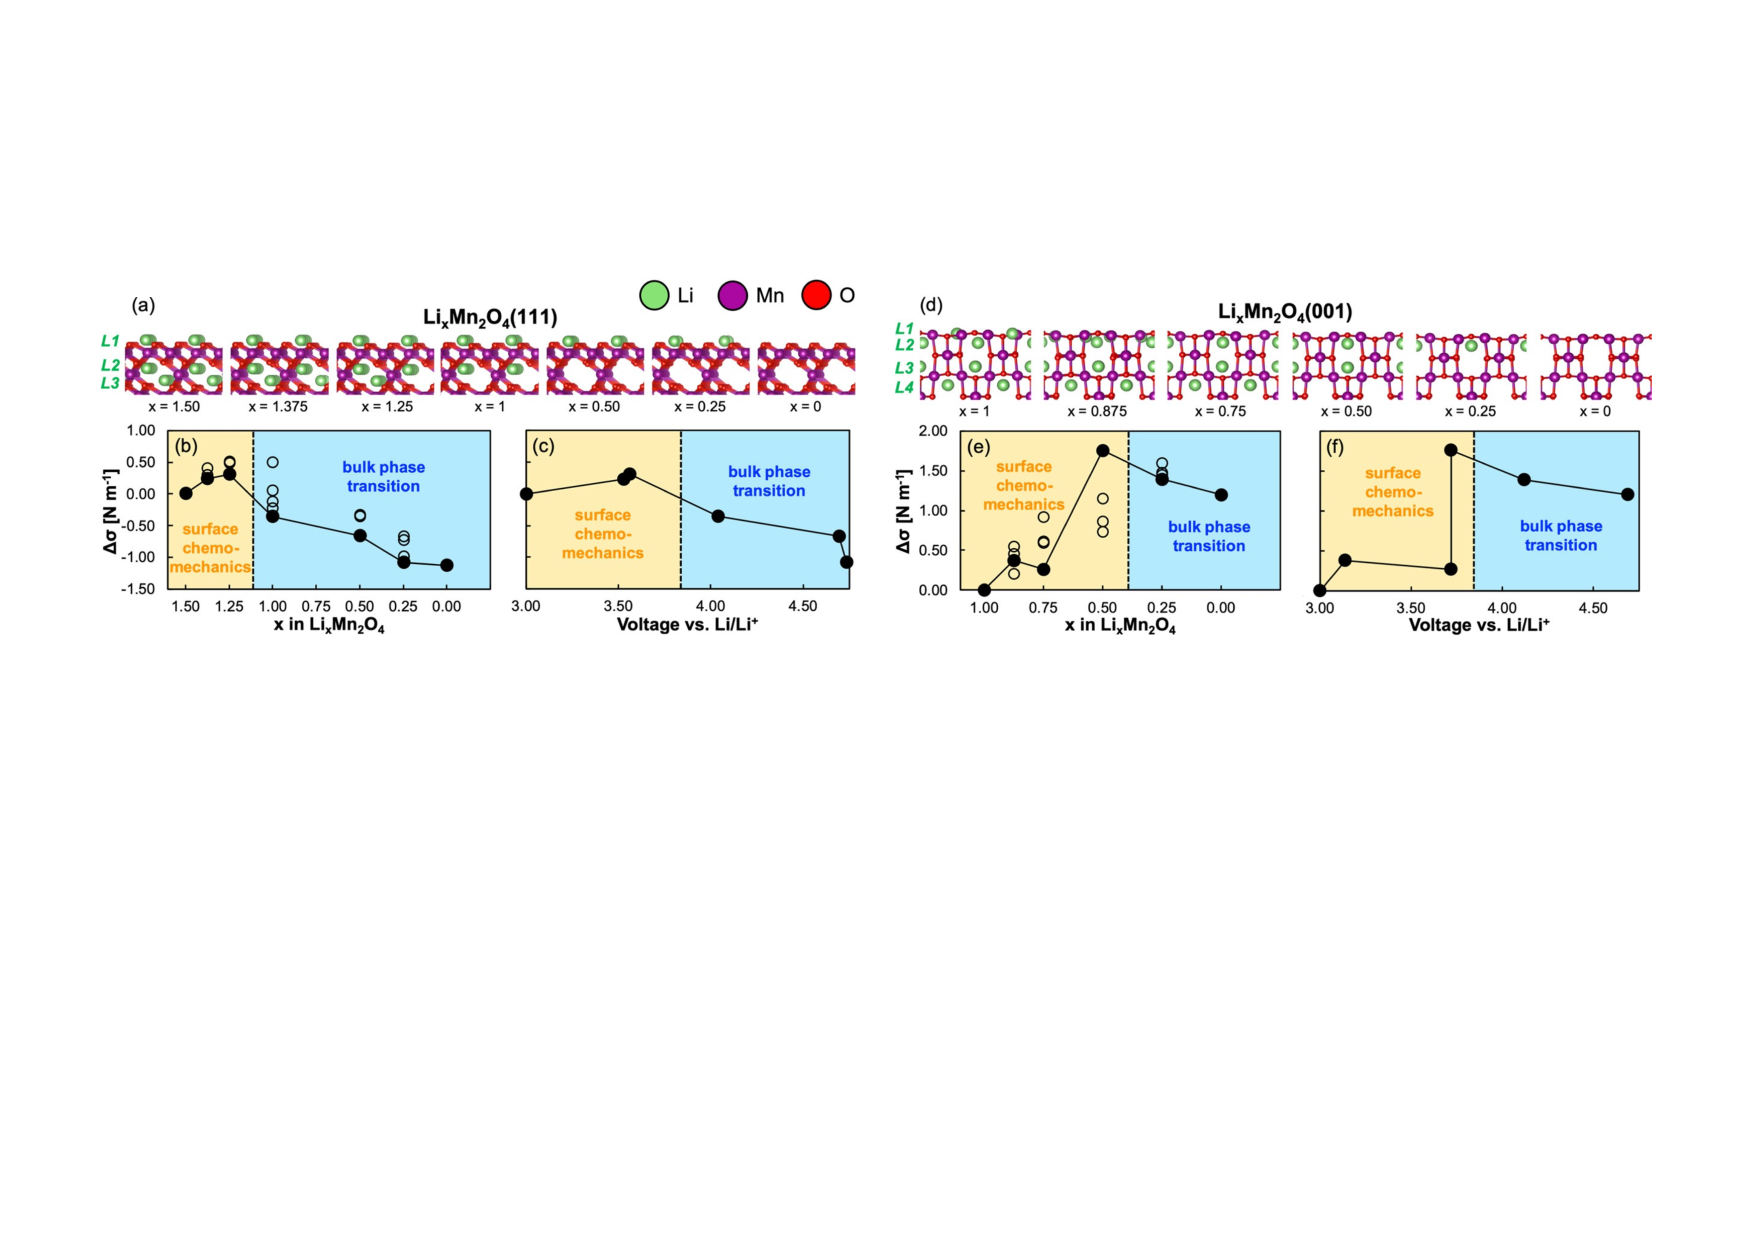
\includegraphics[scale=0.6]{figures/cathode_surface_stress.pdf}
    \caption{Surface stress evolution upon delithiation of lithium manganese oxide (LMO) surfaces. Low energy structures of the (a) LMO(111) and (d) LMO(001) surfaces at different Li$^+$ contents. Differential surface stresses of (b) LMO(111) and (e) LMO(001) as a function of the Li$^+$ content for various Li$^+$ configurations. The filled circles in (b,e) represent the most energetically stable structures for a given stoichiometry. The unfilled circles in (b,e) denote metastable lithium configurations. Differential surface stresses of (c) LMO(111) and (f) LMO(001) as a function of the cell voltage. The dashed lines correspond to the calculated equilibrium potential of 3.84 V vs Li/Li$^+$ between LMO and L$_{0.5}$MO. The yellow-shaded regions correspond to surface-dominated mechanics from the near-surface delithiation. The blue-shaded regions correspond to surface phases that are thermodynamically inaccessible because they become stable only at voltages above the equilibrium potential. Reprinted with permission from Ref~\citenum{warburton2020oriented}. Copyright 2020 American Chemical Society.}
    \label{fig:cathode_surface_stress}
\end{figure}

The surface structures of LiFePO$_4$ exhibit a complex and uneven topology due to the size difference of Li$^+$, Fe$^{2+}$, and PO$_{4}^{3-}$. The majority of terminating surfaces undergo fairly considerable relaxation, which makes predictions based on rigid terminations unreliable. Although LiFePO$_4$ can be synthesised in multiple morphologies exposing different surfaces,\cite{chen2006electron,ellis2007synthesis} studies on the (010) surfaces are particularly interesting. This surface is normal to the most facile pathway for lithium ion conduction, \cite{islam2010recent} reducing the diffusion path lengths for lithium at the surface, enhancing the electrochemical performance of the cathode. DFT calculation of the diffusion pattern and energy landscape of lithium in LiFePO$_4$ showed that the energy barrier for the Li diffusion along (010) is lower than along the other directions, e.g. (100), indicating that the Li diffusion in LiFePO$_4$ is one dimensional.\cite{tankhilsaikhan2019density} Understanding processes such as the lithium (de)intercalation on the LiFePO$_4$ (010) surface is important for developing effective approaches for further improving the material's rate performance. Using DFT calculations, \citeauthor{xu2019insight} found that the extraction of Li from the surface layer has a significant effect on the work function of the LiFePO$_4$ (010) surface, providing evidence for whether Li atoms are present in the outermost layer of LiFePO$_4$ (010) surface or not.\cite{xu2019insight} Here, the authors also calculate the redox potential and formation energies for extracting Li from different (010) surface layers. They find that extracting lithium from the outer surface layers has the lowest redox potential and formation energy, indicating that it is energetically favorable to extract Li first from the surface layer. \citeauthor{xu2019insight} propose a new method that surface work functions can be used for providing insight into the lithium (de)intercalation on the LiFePO$_4$ (010) surface.\cite{xu2019insight}

\citeauthor{zhang2020observation} used a combined experimental and computational (DFT) approach to investigate the preferential cation doping on the surface of LiFePO$_4$ and its effect on properties.\cite{zhang2020observation} The authors found that, for all chosen dopants, there were increased ratios of Fe$^{3+}$/Fe$^{2+}$ oxidation on the particle surfaces, while the core atoms remained closer to that of the pristine, undoped material. This indicates that the dopants are predominantly pushed to the particle surfaces during phase formation. This disparity in distribution of dopant across the core and surface results in improved conductivities.\cite{zhang2020observation} \textit{ab initio} MD simulations with X-ray Diffraction (XRD) and microscopy experiments on the LiFePO$_4$ cathode show Li-ions migrating along the surface, facilitated by solvent molecules.\cite{li2018fluid} This work establishes fluid-enhanced surface diffusion as a key factor in tuning phase transformation in anisotropic solids.

\subsection{Interfaces}
\label{sec:cathode_interfaces}
Although the cathode-electrolyte interphase (CEI) is thinner than the SEI at the anode, it is still quite complex in structure and composition.\cite{Gauthier2015,Edstrom2004} DFT-based simulations can provide insight into adsorption trends,\cite{Bhandari2020} reaction pathways and energetics,\cite{Tebbe2015a, Tebbe2015b} and migration barriers for Li-ion transfer,\cite{Bhandari2019} etc. The electrolyte in a Li-ion battery is typically a Li salt, for example LiPF$_6$ in an organic carbonate solvent, such as ethylene carbonate (EC), propylene carbonate (PC), diethyl carbonate (DEC) or dimethyl carbonate (DMC). The LiPF$_6$ electrolyte reacts with trace amounts of moisture to form hydrofluoric acid (HF),\cite{Tebbe2015a} which is highly corrosive and reacts with the cathode surface to form fluoride-based products.\cite{Tebbe2015b} The organic carbonate solvent also reacts with the cathode surface to form a series of decomposition products.\cite{Tebbe2016} The adsorption of solvent-decomposition and fluoride-based products is the first step in the series of reactions that lead to the formation of the CEI. The decomposition reaction of cyclic organic carbonate solvents proceeds via ring opening, having an energy barrier predicted via climbing image nudged elastic band (CI-NEB) calculations (sections~\ref{sec:dft} and \ref{sec:methods_neb}) to be around 0.62~eV on (100) LiMn$_2$O$_4$ surfaces,\cite{leung2012first} over 1~eV on (101$\Bar{4}$) LiCoO$_2$ surfaces,\cite{Tebbe2016} and around 0.29~eV on (101$\Bar{4}$) Li(Ni,Mn,Co)O$_2$ surfaces\cite{Xu2017}. While experimental studies on the composition of the CEI have shown the presence of both solvent-decomposition and fluoride-based products on most oxide cathodes, such as LiMn$_2$O$_4$, LiNiO$_2$ LiCoO$_2$ and LiNi$_{0.8}$Co$_{0.2}$O$_2$, no solvent reaction or solvent decomposition products are detected on LiFePO$_4$.\cite{Edstrom2004, Malmgren2010} Recent calculations of adsorption energies based on DFT have shown that adsorption preference of HF over EC leads to the entire LiFePO$_4$ nano-particle being covered by fluoride-based products, further leading to their dominant presence in the CEI.\cite{Bhandari2020} DFT simulations have also been used to design suitable coatings in order to prevent cathode degradation.\cite{Tebbe2015b} These calculations can shortlist effective candidate materials to guide experiments. Thus, atomistic methods can not only provide the necessary insights needed in order to explain experimental observations, but also suggest novel solutions for mitigating cathode degradation.

Apart from the complexity of structure of the CEI, another challenge is understanding Li-ion migration at the CEI, impacting the rate capability of LiBs. Li-ion conductivity in bulk electrolyte is around 1 S cm$^{-1}$ (c.f. section~\ref{sec:electrolytes}) which is several orders of magnitude higher than that in bulk electrode materials (c.f. sections~\ref{sec:anodes_ion_diffusion} and \ref{sec:cathode_ion_diffusion}) (around 10$^{-7}$--10$^{-2}$ S cm$^{-1}$).\cite{park2010review, VanDerVen2013} However, the complex structure of the CEI and uncertainty about the mechanism of Li-ion transfer across it has hindered the understanding of kinetics at the interface. Recent NEB calculations on the LiFePO$_4$ cathode have estimated an energy barrier of 756~meV, for Li to move from a near-surface solvated cluster to a sub-surface vacancy in the LiFePO$_4$ cathode material.\cite{Bhandari2019} Due to preferential adsorption of fluoride on LiFePO$_4$ surfaces,\cite{Edstrom2004,Bhandari2020} the energy barrier has been found to decrease to 410~meV in the presence of fluoride. Nevertheless, the interfacial energy barrier is higher than that in bulk cathode material, which is estimated to be around 270--290~meV.\cite{Morgan2004,Dathar2011} This highlights a rate-limiting behaviour of the interface in the overall Li-ion diffusion process in LiBs. This study motivates further investigation on other cathode electrolyte interfaces, especially with recently developed advanced methods for characterising the interface, as described in section~\ref{sec:dft+cont}.

\subsection{Outlook and challenges for cathodes}
\label{sec:cathodes_outlook}
%NMC materials and Li-rich
Lowering the cost, increasing capacity, and improving the sustainability of battery materials is becoming more critical, as we move towards large-scale deployment of LiBs for applications such as EVs.\cite{dunn2011electrical} Here, we highlight some of the outstanding challenges for cathodes and how atomistic modelling can provide insights and suggest solutions.

Ni-rich NMC layered oxides are favorite candidates for cathode materials, due to their high gravimetric and volumetric energy densities.\cite{li2020high} However, these materials have three critical challenges: cycle instability, thermal instability, and air instability. These are all linked with the instability of Ni$^{3+}$ and Ni$^{4+}$ at the surface/interface. Other cathode materials, such as oxyfluorides, have worked towards solving some of these issues, however, there are still outstanding surface and interfacial challenges, for which atomistic modelling is vital:

\begin{itemize}
    \item In Ni-rich NMC, the unstable Ni$^{3+}$ and Ni$^{4+}$ react aggressively with the electrolyte to form thick CEI layers and cause Ni and Mn dissolution. The dissolute TMs then migrate to the anode and cause electrolyte decomposition, leading to thick SEI layers which limit the battery cyclability.\cite{li2017dynamic,li2018mn} CEI and SEI formation are crucial challenges to be overcome for both conventional and solid-state batteries. \hlcyan{Although electrochemical spectroscopic techniques have been used to obtain molecular scale information, further detail, which cannot be resolved using current experimental techniques, is needed to gain more reliable information.}\cite{middlemiss2020characterisation} \hlcyan{For example, deconvoluting impedance components in two-terminal electrochemical impedance spectroscopy (EIS) data for materials that have similar time constants, such as solid-state lithium charge transfer in a cell with a graphitized carbon anode and LiCoO$_2$ cathode, is challenging.}\cite{li2001studies} \hlcyan{Half-cell measurements can be used to study the impedance of the two electrodes separately, but these measurements do not fully reflect the processes occurring in a full-cell battery at different states of (dis)charge.}\cite{song2002two} \hlcyan{Three-electrode cell configurations present a way to potentially disentangle the impedance components from the anode and cathode.}\cite{li2001studies} \hlcyan{However, these measurements are fraught with uncertainties, as the insertion of the reference electrode can fundamentally change the electrochemistry.}\cite{McTurk_2015,Belt_2014} \hlcyan{This is where atomistic modelling is well suited to provide the fundamental understanding of the limiting rate constants in electrochemistry, that can be used to guide further experiments. As available experimental techniques are unable to provide significant insight into the atomistic mechanism of Li-ion transfer at the cathode-electrolyte interface, atomistic modelling is ideally suited to shed light in this area. For example,} \citeauthor{Bhandari2019} \hlcyan{used DFT to investigate the interfacial Li-ion transfer mechanism at an atomic level, from bulk ethylene carbonate (EC)/LiPF$_6$ electrolyte into a LiFePO$_4$ cathode, and provide an estimate on the corresponding energy barrier.}\cite{Bhandari2019}
    \item Phase transitions at the surface of cathode materials occur at a high state of charge and affect the surface reactivity, resulting in increased TM dissolution and CEI/SEI formation. The effect of this is rapid capacity fading during cycling.\cite{li2019comprehensive} Co-free Li-rich layered oxides, such as Li[Li$_{0.2}$Mn$_{0.6}$Ni$_{0.2}$]O$_{2}$, are appealing due to their low cost and high capacities (300 mAh g$^{-1}$).\cite{kim2004electrochemical,armstrong2006demonstrating} However, these materials undergo layered to spinel transitions due to low octahedral site stability of Mn$^{3+}$, leading to voltage decay during cycling and Mn dissolution,\cite{MnDissolution2016} making these materials challenging to employ as a practical cathode. Atomistic insight into the mechanisms involved in these phase transitions, gained through \textit{ab initio} and potentials-based MD methods, can provide the detail and understanding needed to prevent these phase transitions from occurring.
    % O redox & O2 formation rewrite
    \item Some cathode materials show reversible O-redox, with lower voltage hysteresis and, where O$_2$ is formed, it reincorporates into the lattice.\cite{Sharpe2020} In contrast, other materials show irreversible O-redox, with O$_2$ lost from the surface,\cite{Nakayama2020, Chen2016, House2020a} leading to unwanted side reactions with the electrolyte. The formation and potential loss of molecular O$_2$ is likely to be heavily dependent on local structure. In the case of Li$_2$MnO$_2$F, DFT showed that O$_2$ is formed only in O-Li rich areas, not in O-Mn rich areas.\cite{Sharpe2020} Meanwhile, other oxyfluorides, such as Li$_2$VO$_2$F, do not show molecular O$_2$ formation at all, but instead form superoxides on charging.\cite{Chang2020} 
\end{itemize}

It is challenging to model disordered systems as, by their very nature, they can have an almost infinite arrangement of atoms. Use of computational techniques, such as cluster expansion, to generate low energy structures of disordered rock-salts, is a promising route to more realistic DFT studies.\cite{Lun2020}

%Interatomic potentials
As discussed in sections~\ref{sec:potential_fitting} and \ref{sec:electrolyte_classicMD}, more careful considerations of the factors/parameters to include when fitting interatomic potentials for a system is key to improving the quality of research conducted through potentials-based modelling. It is commonplace to reuse potentials from literature sources, without determining how they were fitted, which can lead to inaccuracies in the calculations performed. For example, if the potentials for a cathode material were fitted only to lattice parameters, elastic constants, and the bulk modulus, then the potential would not be accurately representative of the cathode redox properties. If properties such as the dielectric constant were included, then redox chemistry would be better represented. In effect, interatomic potentials in literature are not necessarily transferable to different types of study. It is not feasible to fit to every material property, however, a broader range of properties, most relevant to the study being conducted, is required. There are tools in development \cite{gale_empirical_1996, Stukowski_2017, wen_kim-compliant_2017, Morgan2021PopOff} aiming to make this potential fitting process more accessible to atomistic modellers, with the ability to fit to a larger range of parameters. However, there is still a need for improved transparency in the publication of studies using interatomic potentials. Use of machine learning to develop potentials has also shown to be a promising avenue. \citeauthor{deringer2019machine} recently published a progress update, showing how machine learning is improving interatomic potentials by ``learning'' from electronic-structure data, giving increased accuracy in approximating material properties.\cite{deringer2019machine}

%concluding statement
In-depth insight into the elemental distribution, electronic structure, and crystalline structure under electrochemical conditions is challenging to achieve experimentally. Atomistic techniques, including DFT and MD, are well suited to provide the insight needed for these properties. However, future research and development of cathode materials will require collaborative efforts, involving the disciplines of chemistry, physics, material science, nanoscience/nanotechnology, and computational modelling/simulation.\cite{yu2018electrode}
\end{document}